\subsection{Recurrent neural networks}
\label{section:BT:RNN}

A \textbf{Recurrent Neural Network (RNN)}is an artificial neural network architecture that can work with data sequences of arbitrary length.
Unlike feed-forward networks, RNNs consider the input data in conjunction with state information from a previous timestep.
To accomplish this, the network uses feedback connections.
The feedback connections serve state information from the previous time step to the intended node.
This connection works as a short-term memory for the recurrent layers, saving information from the previous time step memory cells.

In the basic RNN, these memory cells retain minimal information, saving data only from the previous instance.
As the RNN memory cell is defined by the newest data introduced to the cell, previous information is encoded only in its effect on that data.
Due to this, information is not stored for long in these memory cells, only retaining short-term memory data.

The RNN is able to process data of arbitrary length, meaning that it is well suited for natural language processing, time-series analysis, and similar problems.
In addition, the memory retained in the RNN makes it well suited to extract temporal relations in the data.

\begin{figure}[h!]
  \centering
  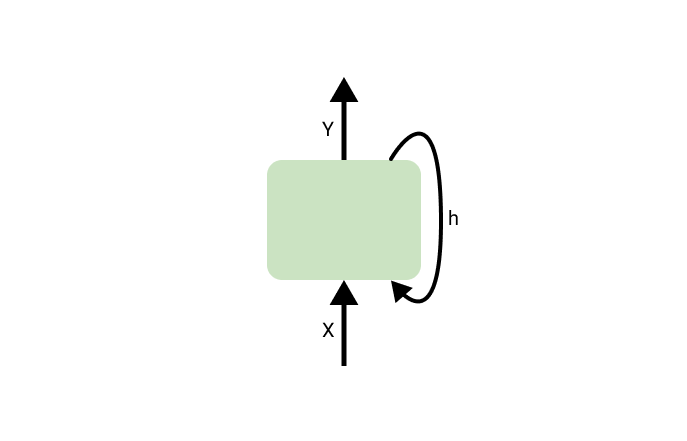
\includegraphics[width=0.5\textwidth]{./sections/BT/figures/RNN.png}
  \hfill
  \caption{Figure of RNN feedback-cell.}
  \label{fig:rnn-cell}
\end{figure}



In order to improve the performance of the RNN, new models have been created to address some of its shortcomings.
One such model is the Long-Short Term Memory model (LSTM) \cite[p.~469-472]{Geron2017}.


\subsection{Long-Short Term Memory}
\label{section:BT:LSTM}

\textit{Long-Short Term Memory} (LSTM) is a type of recurrent neural network addressing some of its shortcomings
The LSTM introduces a new memory cell, adding Long-term memory to the network.

The LSTM memory cells are comprised of two vectors, one for long-term and one for short-term memory,
as well as an input gate, output gate, and a forget gate.
The forget gate allows for the memory cell to remove unneeded parts of the memory in order to replace it with new data from the input gate.
The long-term memory retains some of its information while replacing other parts.

The long-term memory of the LSTM enables it to solve the RNN problem of vanishing gradients.
The long-term memory enables the LSTM to store data at arbitrary intervals, as well as to detect long-term dependencies in the data.

The LSTM, like the RNN, is well suited for working on a series of data.
The LSTM can analyze and predict long-term relations in a series of data, making it well suited for applications such as time-series prediction or anomaly detection,
natural language processing, and more
\cite[p.~492-493]{Geron2017}.

\begin{figure}[h!]
  \centering
  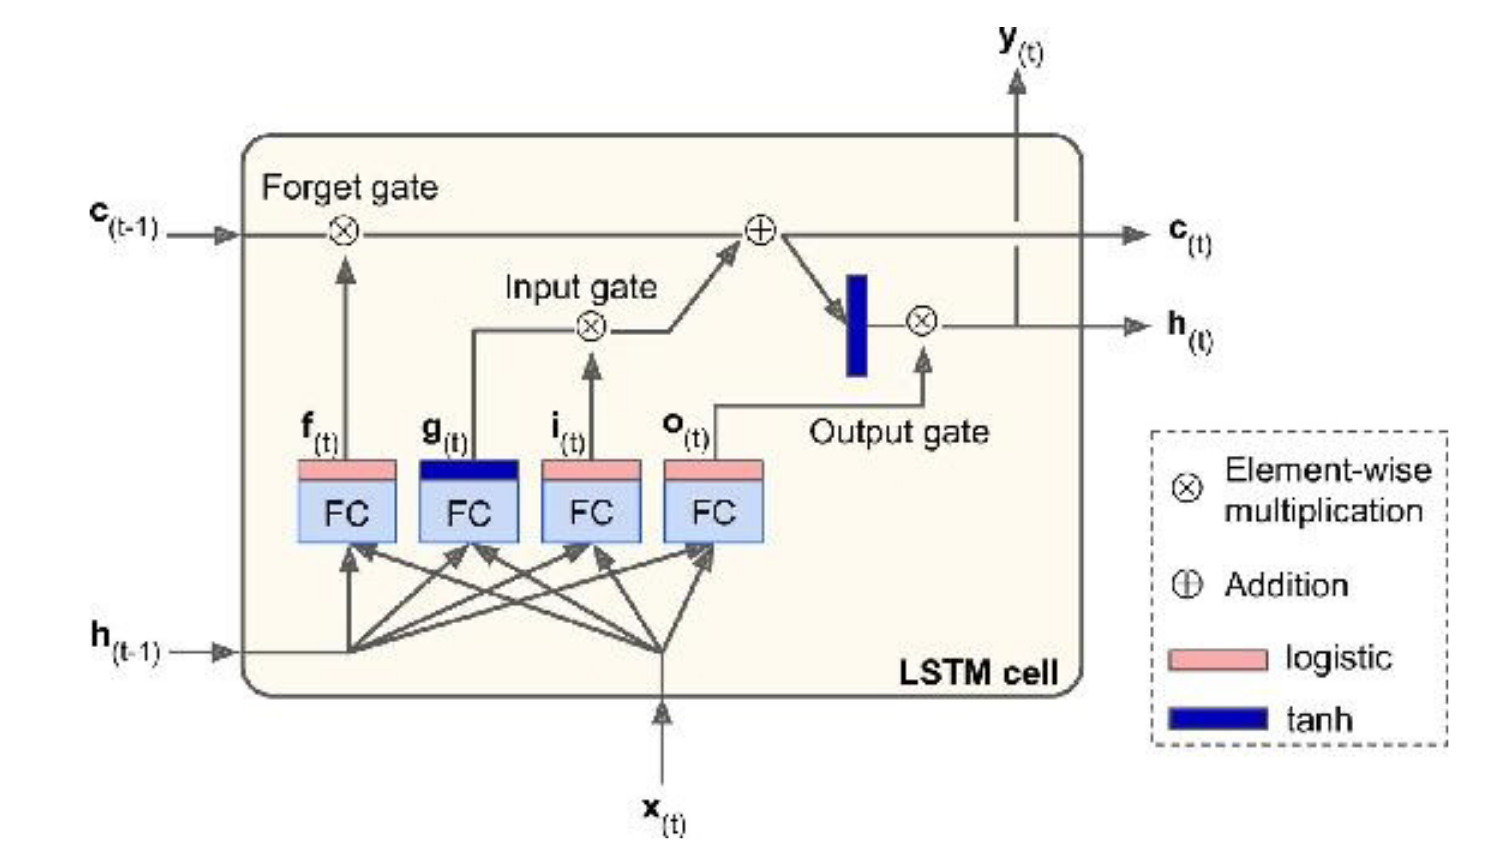
\includegraphics[width=0.7\textwidth]{./sections/BT/figures/lstm_cell_hands_on.png}
  \hfill
  \caption{Figure of LSTM memory cell from \cite[p.~492]{Geron2017}.}
  \label{fig:lstm-memory-cell}
\end{figure}



% [ Legge til Wikipedia kilde? ]

\subsection*{Stateful and stateless LSTMs}
\label{section:BT:stateful-vs-stateless}
An LSTM takes three vectors as input. The hidden previous hidden state $H_{t-t}$
which is the short term vector described above, the previous cell state
$C_{t-1}$ which is the long term vector, and the input vector $X_t$.
These are not to be confused with the cells internal weights $W_i$
which is the weight matrix for the hidden state vector, and $U_t$,
the weight matrix for the input $X_t$.

During training these weight matrixes are shaped by backpropegation.
The hidden state and internal state vectors are not touched by backpropegation,
but will be constantly changing during forward passes through the network.

A stateful LSTM refers to an architecture where the hidden state and cell state
are initialized once but never reset during training. This is typically
when the batches in the training set are dependent on each other, like
one long time series.

In a stateless LSTM the hidden states are reset many times during training,
typically at the end of each batch. A typical example is if the training
data is a set of unrelated sentences.


